% Created 2023-04-04 Tue 00:01
% Intended LaTeX compiler: lualatex
\documentclass[bigger]{beamer}
\usepackage{graphicx}
\usepackage{longtable}
\usepackage{wrapfig}
\usepackage{rotating}
\usepackage[normalem]{ulem}
\usepackage{amsmath}
\usepackage{amssymb}
\usepackage{capt-of}
\usepackage{hyperref}
\usetheme[progressbar=foot, sectionpage=none, numbering=fraction]{metropolis}
\usepackage{tikz}
\usepackage{booktabs}
\usepackage{adjustbox}
\usepackage{diagbox}
\usepackage{latexcolors}
\usetikzlibrary{automata, positioning, arrows, arrows.meta}
\usepackage{diagbox}
\usepackage{dsfont}
\usepackage{fontawesome5}
\usepackage{color}
\usepackage{transparent}
\usepackage{tcolorbox}
\usepackage[absolute, overlay]{textpos}
\setlength{\TPHorizModule}{\textwidth}
\setlength{\TPVertModule}{\textwidth}
\usepackage{enumitem}
\setlist[itemize]{label=\textbullet}
\usepackage{mathtools}
\usepackage[mathrm=sym]{unicode-math}
\definecolor{RedBrown}{RGB}{192, 4, 4} \setbeamercolor{progress bar}{fg=RedBrown} \setbeamercolor{title separator}{fg=RedBrown}
\setbeamercolor{progress bar in head/foot}{fg=RedBrown} \setbeamercolor{progress bar in section page}{fg=RedBrown} \setbeamercolor{alerted text}{fg=RedBrown}
\pretocmd{\tableofcontents}{\thispagestyle{empty}}{}{}
\addtocounter{framenumber}{-1}
\usepackage{listings}
\usepackage{xcolor}
\definecolor{codegreen}{rgb}{0,0.6,0}
\definecolor{codegray}{rgb}{0.5,0.5,0.5}
\definecolor{codepurple}{rgb}{0.58,0,0.82}
\definecolor{backcolour}{HTML}{f0f0f0}
\lstdefinestyle{mystyle}{
backgroundcolor=\color{backcolour},
commentstyle=\color{codegreen},
keywordstyle=\color{magenta},
numberstyle=\tiny\color{codegray},
stringstyle=\color{codepurple},
basicstyle=\ttfamily,
breakatwhitespace=false,
breaklines=true,
captionpos=b,
keepspaces=true,
numbers=none,
numbersep=5pt,
showspaces=false,
showstringspaces=false,
showtabs=false,
tabsize=2
}
\lstset{style=mystyle}
\usetheme{default}
\author{Andrea Pierré}
\date{April 4, 2023}
\title{Learning useful representations to solve a place-odor association task}
\institute{Fleischmann Lab}
\titlegraphic{\hfill
\includegraphics[height=1.5cm]{img/Brown Logo_2016_2 Color Process ST_1300.png}\vspace{8em}\flushright
\includegraphics[height=1.5cm]{img/qr-code.png}}
\setbeamercovered{transparent=10}
\hypersetup{
 pdfauthor={Andrea Pierré},
 pdftitle={Learning useful representations to solve a place-odor association task},
 pdfkeywords={},
 pdfsubject={},
 pdfcreator={Emacs 28.2 (Org mode 9.6)}, 
 pdflang={English}}
\begin{document}

\maketitle
\section*{Collaborators}
\label{sec:org94d245d}
\begin{frame}[label={sec:org3e758c5},plain]{Collaborators}
%\addtocounter{framenumber}{-1}
\begin{adjustbox}{max width=\textwidth, keepaspectratio}
\begin{minipage}[t]{0.2\textwidth}
\center
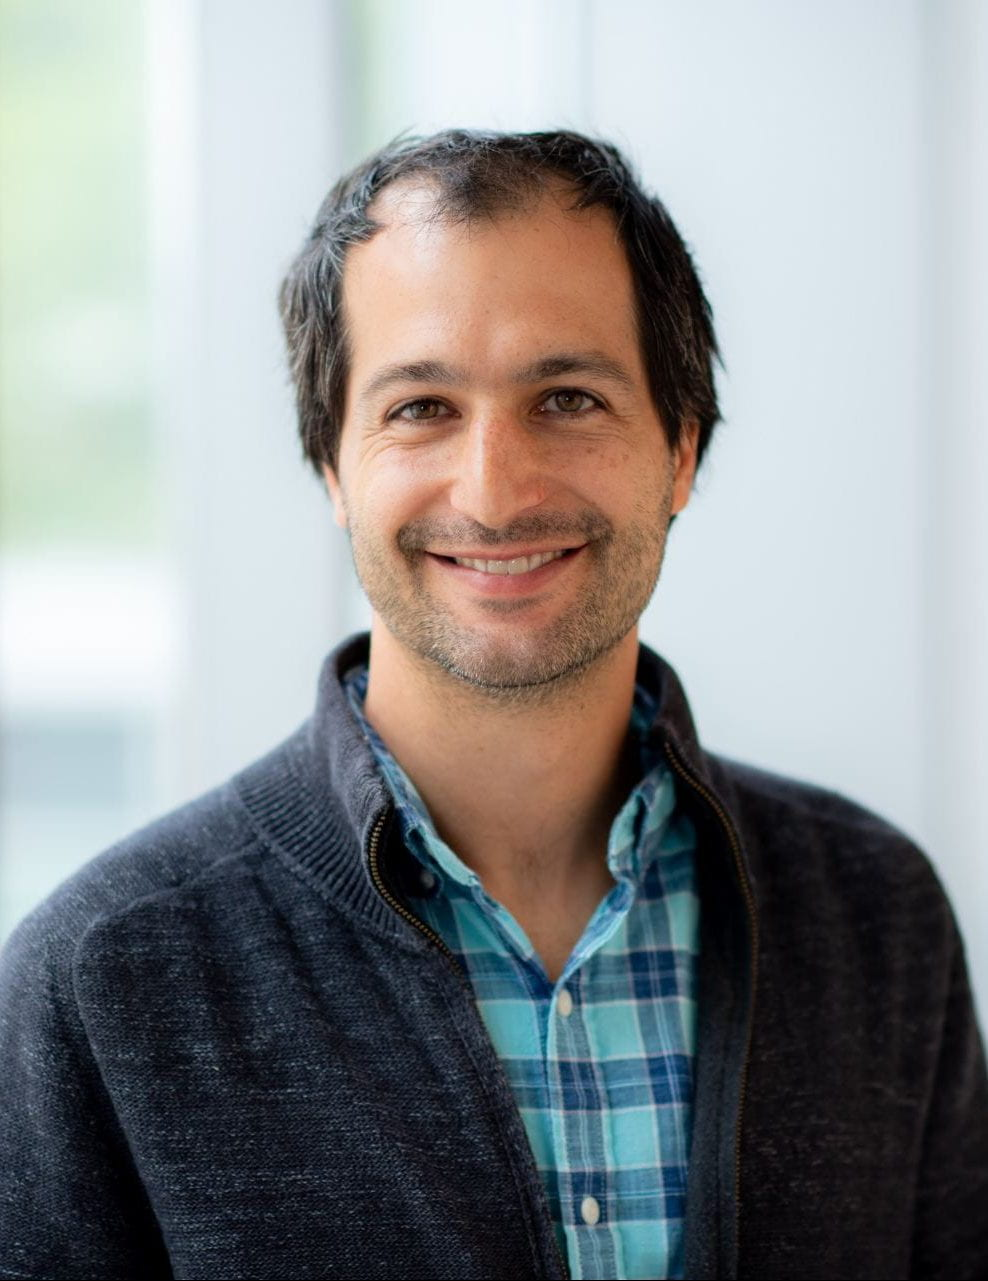
\includegraphics[height=0.2\textheight]{img/matt-nassar.jpg}\\
\scriptsize
Matt Nassar
\end{minipage}
\begin{minipage}[t]{0.2\textwidth}
\center
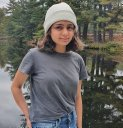
\includegraphics[height=0.2\textheight]{img/niloufar-razmi.jpeg}\\
\scriptsize
Niloufar Razmi
\end{minipage}
\begin{minipage}[t]{0.2\textwidth}
\center
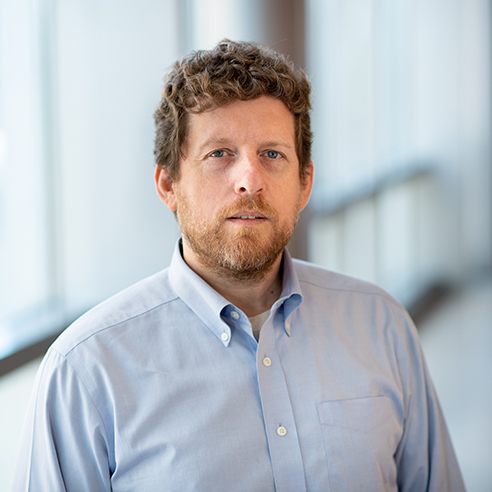
\includegraphics[height=0.2\textheight]{img/jason-ritt.jpg}\\
\scriptsize
Jason Ritt
\end{minipage}
\begin{minipage}[t]{0.2\textwidth}
\center
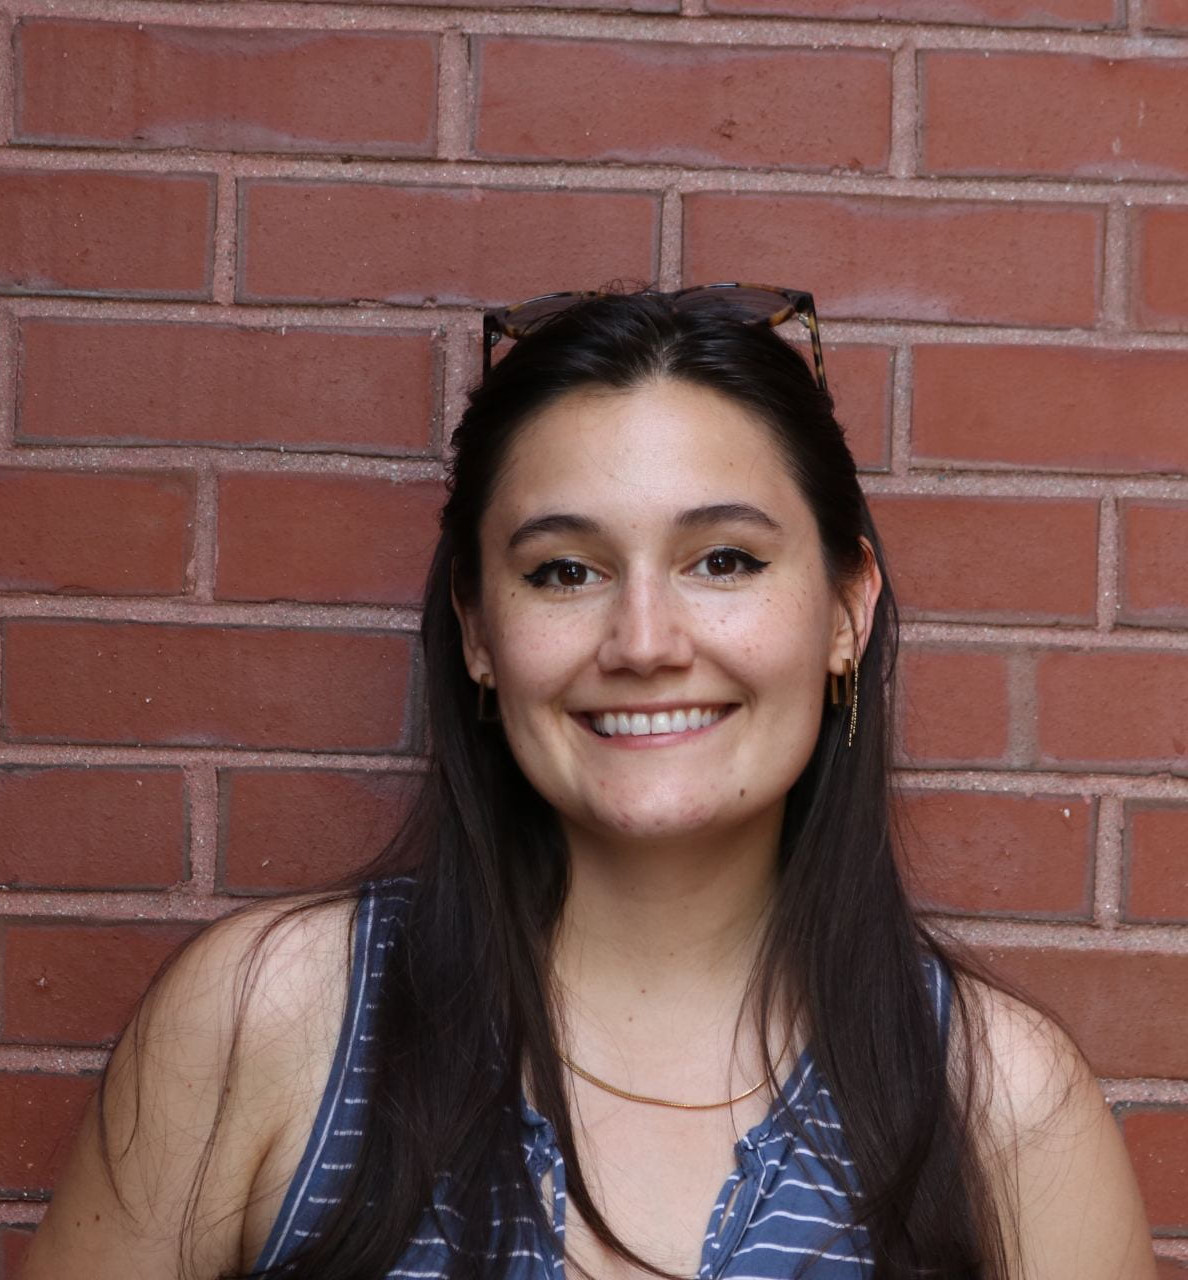
\includegraphics[height=0.2\textheight]{img/olivia.jpg}\\
\scriptsize
Olivia McKissick
\end{minipage}
\begin{minipage}[t]{0.2\textwidth}
\center
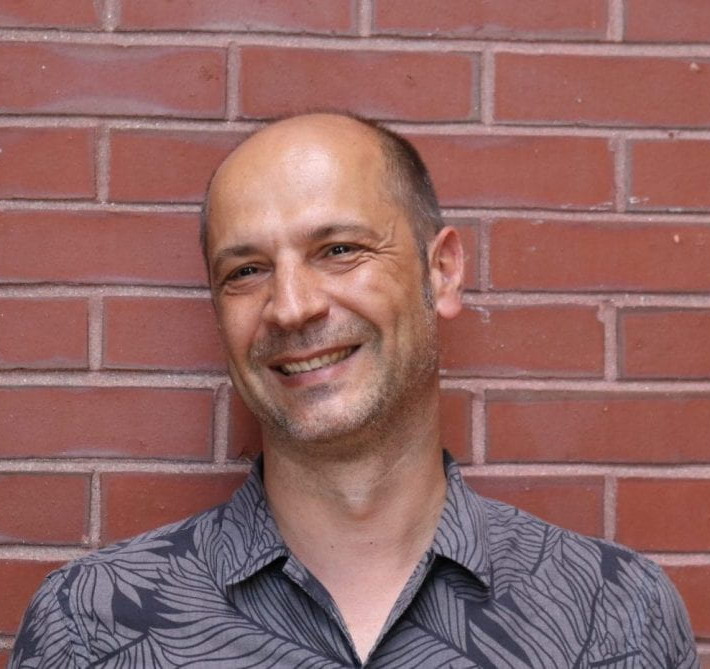
\includegraphics[height=0.2\textheight]{img/alex-fleischmann.jpg}\\
\scriptsize
Alex Fleischmann
\end{minipage}
\end{adjustbox}
\end{frame}
\section*{Context}
\label{sec:orgbb8c3eb}
{%
\setbeamertemplate{background canvas}{\includegraphics[height=\paperheight]{img/rooms1.svg.png}}
\begin{frame}[fragile]{Odor-place association}
\end{frame}
}
\section*{Context}
\label{sec:org47883fb}
{%
\setbeamertemplate{background canvas}{\includegraphics[height=\paperheight]{img/rooms2.svg.png}}
\begin{frame}[fragile]{Odor-place association}
\addtocounter{framenumber}{-1}
\end{frame}
}
\section*{Context}
\label{sec:orge0a6f3f}
\begin{frame}[label={sec:org2d5aee1}]{The LEC is key to sensory associations and spatial memory}
\begin{columns}
\begin{column}{0.45\columnwidth}
%\pause
%\scriptsize
%\footnotesize
\footnotesize
\begin{itemize}
\item \alert{Piriform} encodes olfactory information
\item \alert{Hippocampus} encodes spatial information
\item \alert{Lateral Entorhinal Cortex (LEC)} encodes both olfactory \& spatial information
\end{itemize}
\end{column}
\begin{column}{0.55\columnwidth}
\begin{center}
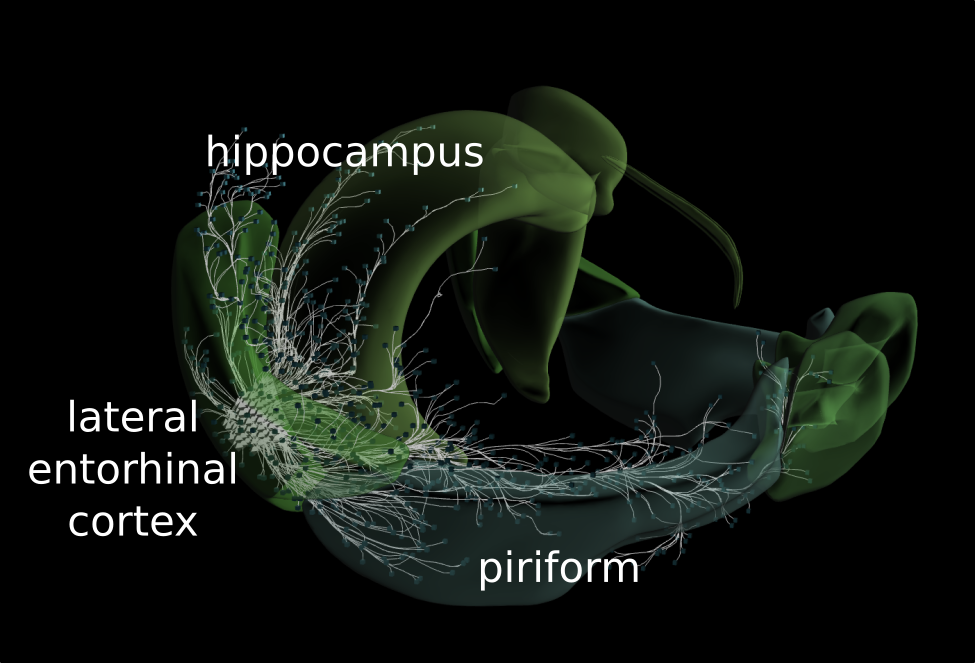
\includegraphics[width=\textwidth]{img/brain.png}
\end{center}
\end{column}
\end{columns}
\end{frame}

\begin{frame}[label={sec:org9a4134e}]{Diamond arena experimental setup}
\begin{textblock}{0.2}(1,0.071)%
\center
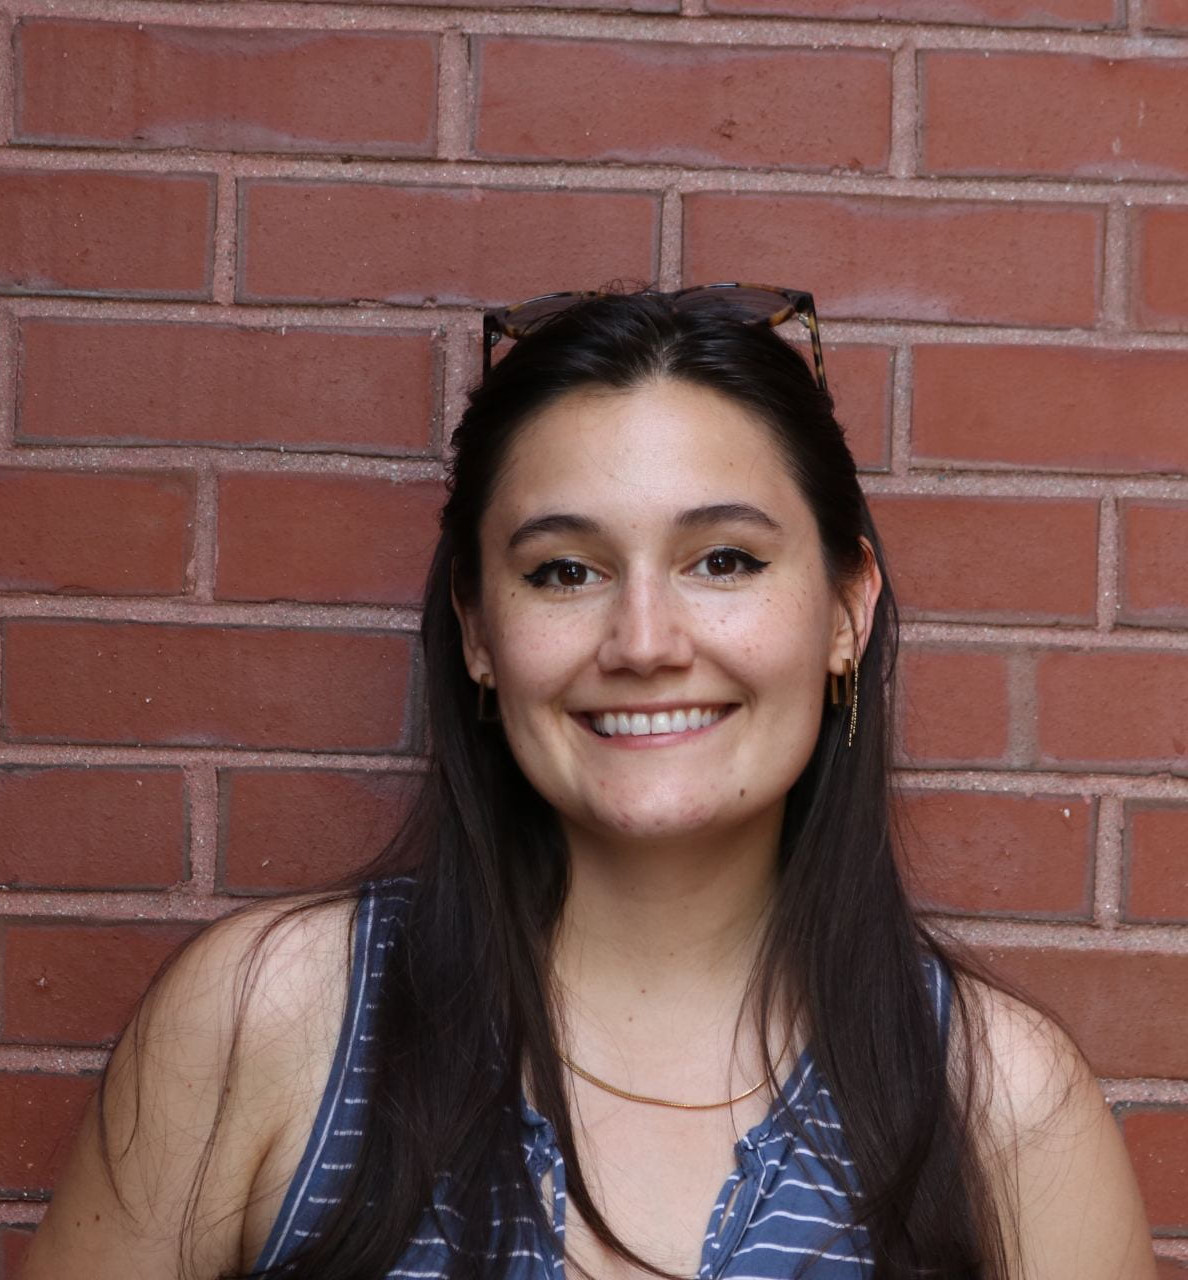
\includegraphics[width=3em]{img/olivia.jpg}\\
\scriptsize
Olivia\\McKissick
\end{textblock}
\begin{center}
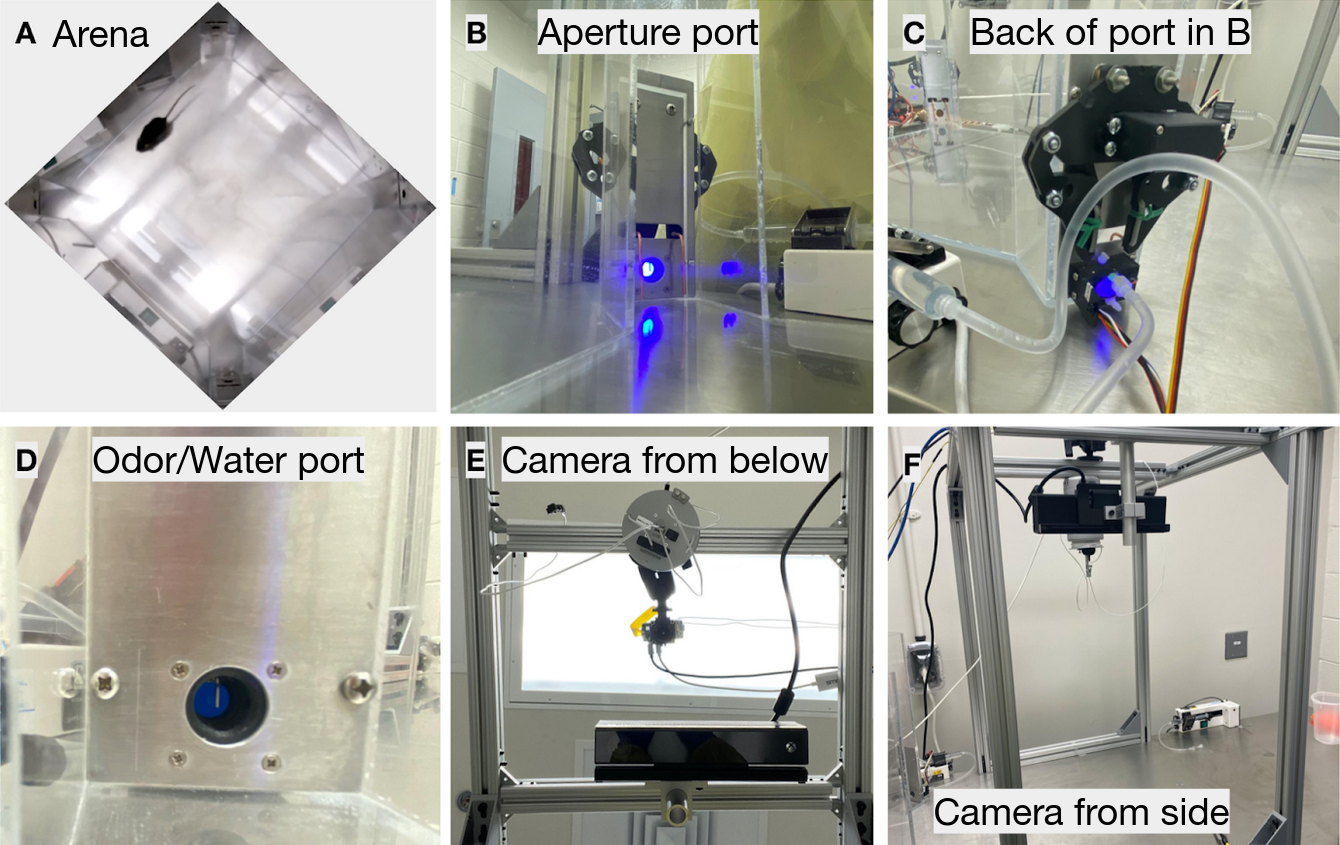
\includegraphics[width=0.8\textwidth]{img/physical-diamond-arena.png}
\end{center}
\(\to\)~1P calcium imaging recording on freely moving mice
\end{frame}
\begin{frame}[label={sec:org21e64f9}]{Diamond arena olfactory task}
\begin{textblock}{0.2}(1,0.071)%
\center%
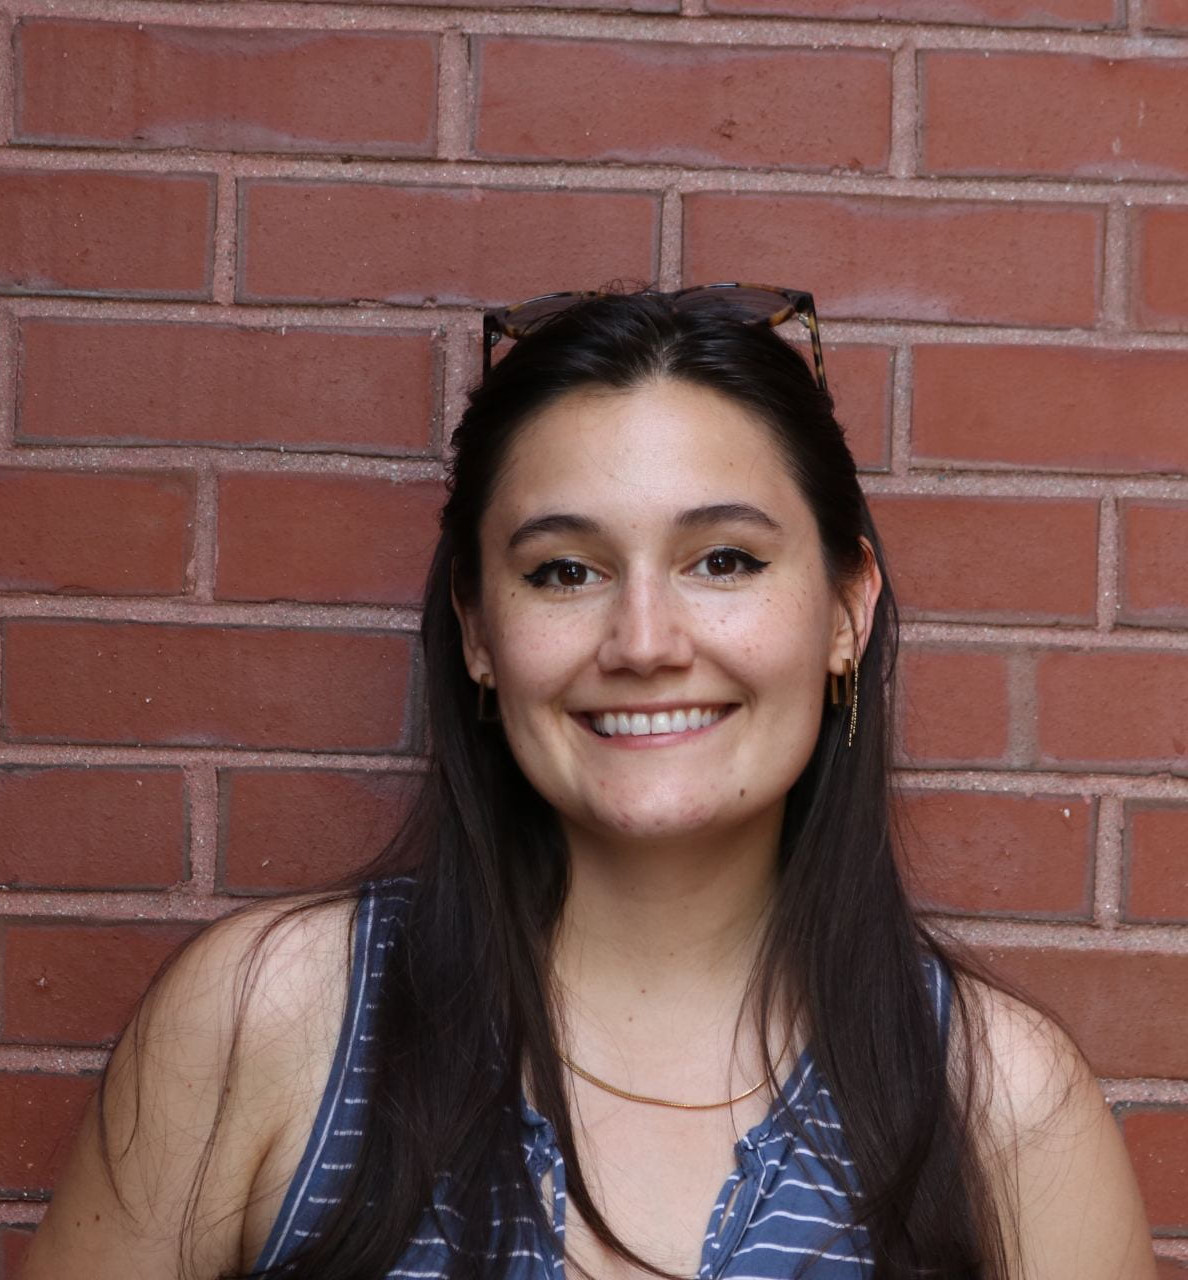
\includegraphics[width=3em]{img/olivia.jpg}\\
\scriptsize
Olivia\\McKissick
\end{textblock}
\begin{columns}
\begin{column}[t]{0.5\columnwidth}
\center
\vspace{-2em}
Allocentric\\
(go west/east)
\vspace{-1.5em}
\begin{center}
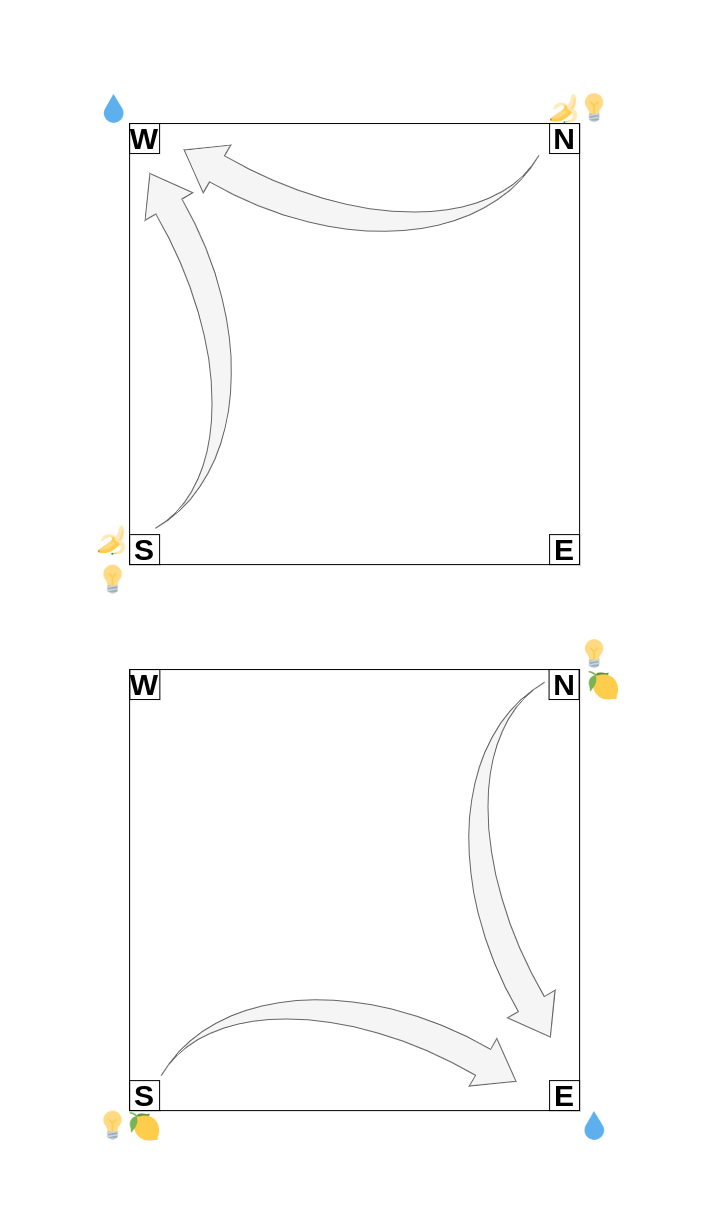
\includegraphics[width=0.8\textwidth]{img/RL_env-allo-task.drawio.png}
\end{center}
\end{column}
\begin{column}[t]{0.5\columnwidth}
\end{column}
\end{columns}
\end{frame}
\begin{frame}[label={sec:org6ae2186}]{Diamond arena olfactory task}
\addtocounter{framenumber}{-1}
\begin{textblock}{0.2}(1,0.071)%
\center%
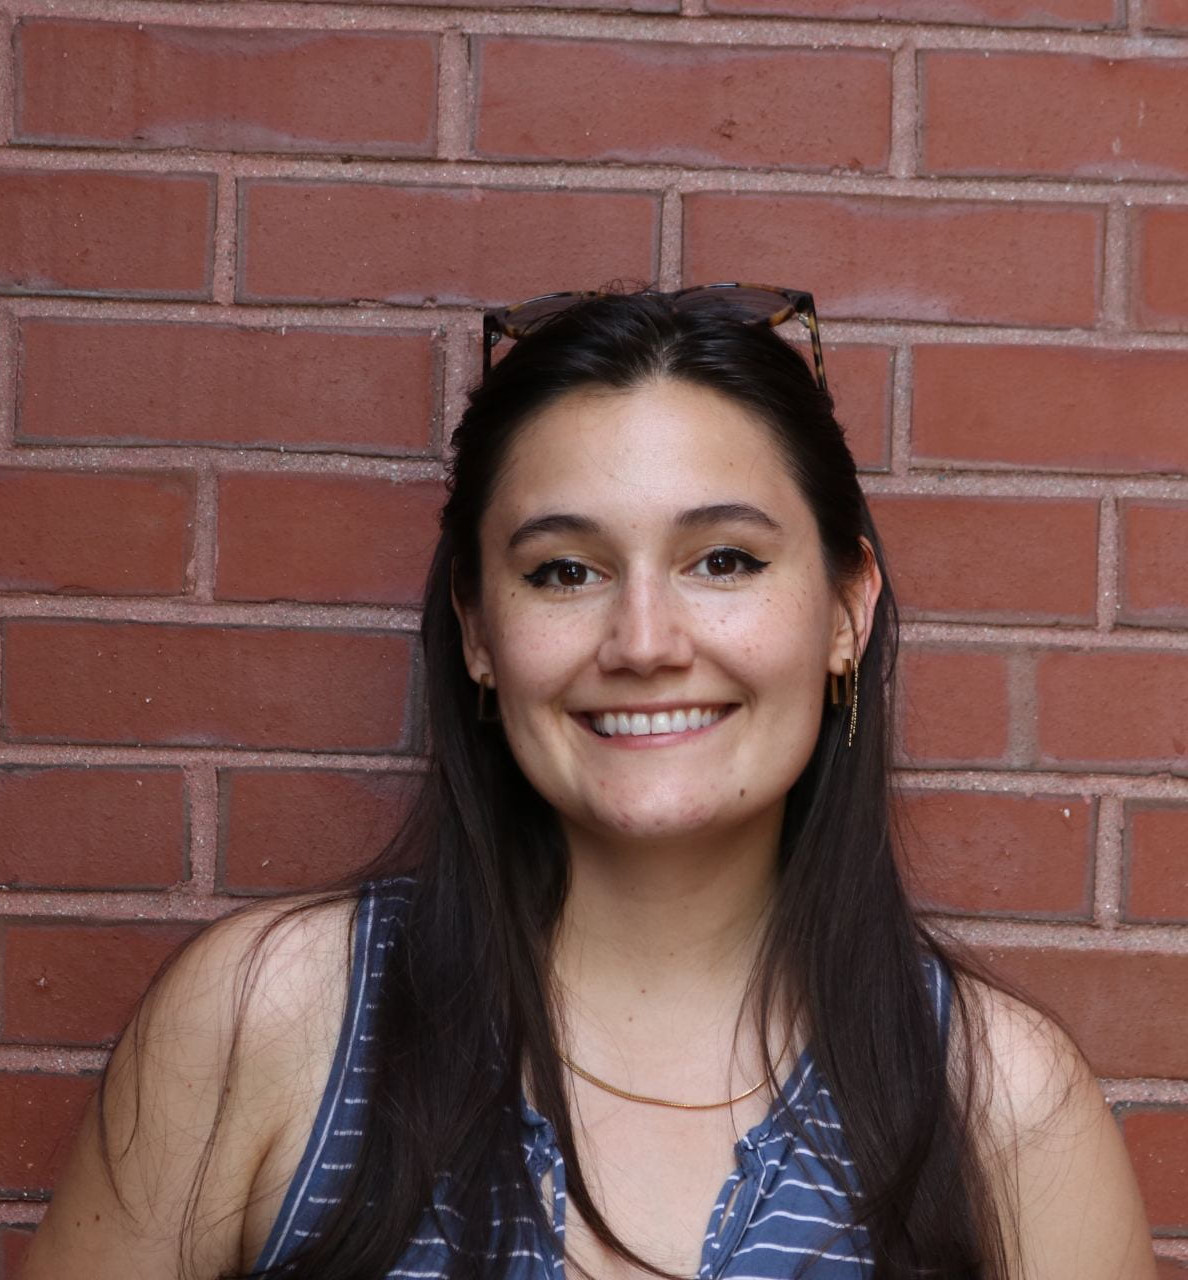
\includegraphics[width=3em]{img/olivia.jpg}\\
\scriptsize
Olivia\\McKissick
\end{textblock}
\begin{columns}
\begin{column}[t]{0.5\columnwidth}
\center
\vspace{-2em}
Allocentric\\
(go west/east)
\vspace{-1.5em}
\begin{center}
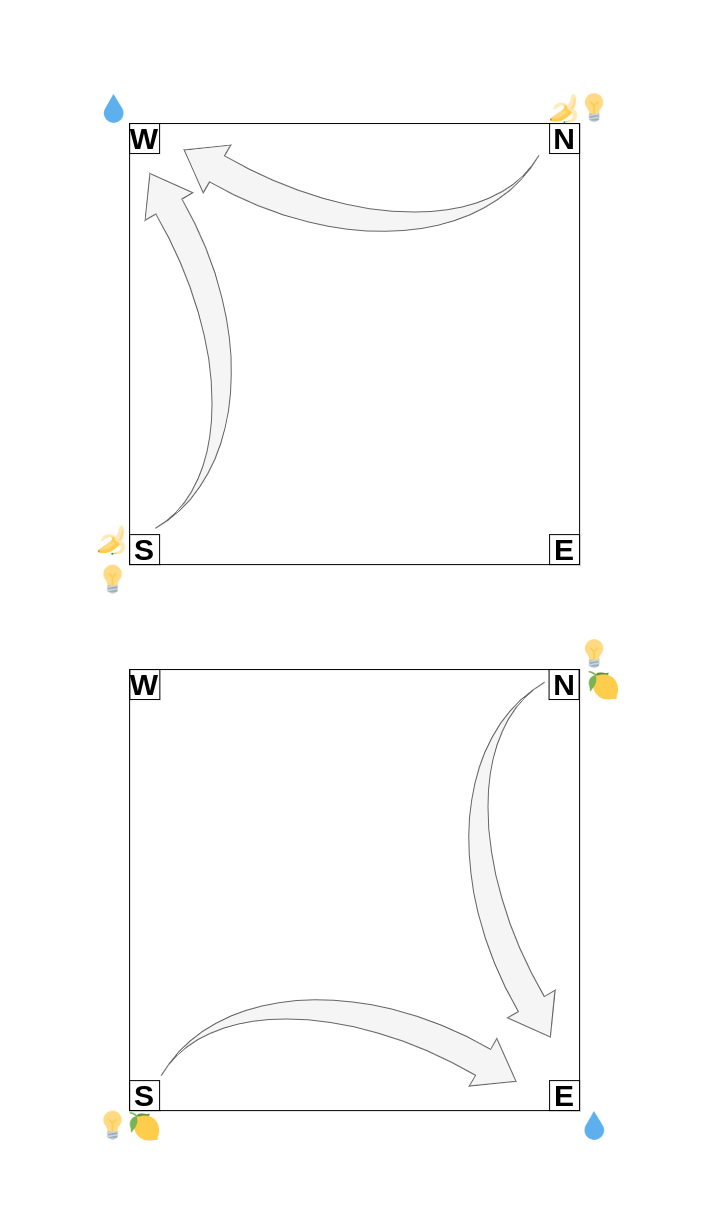
\includegraphics[width=0.8\textwidth]{img/RL_env-allo-task.drawio.png}
\end{center}
\end{column}
\begin{column}[t]{0.5\columnwidth}
\center
\vspace{-2em}
Egocentric\\
(go right/left)
\vspace{-2em}
\begin{center}
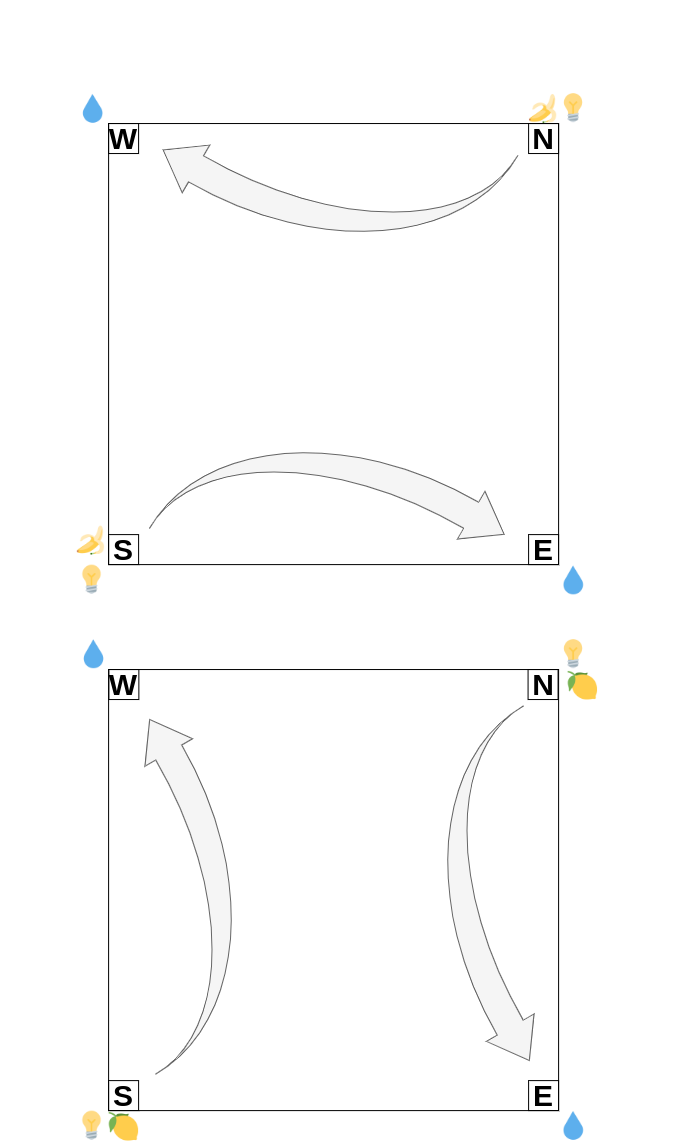
\includegraphics[width=0.8\textwidth]{img/RL_env-ego-task.drawio.png}
\end{center}
\end{column}
\end{columns}
\end{frame}
\begin{frame}[<+->][label={sec:org33182db}]{What is Reinforcement Learning and why use it ?}
\begin{columns}
\begin{column}{0.55\columnwidth}
% \usepackage{fontawesome5}
\usetikzlibrary{positioning,fit,arrows}


\tikzset{
    %Define standard arrow tip
    >=latex,
    %Define style for boxes
    punkt/.style={
           rectangle,
           rounded corners,
           draw=black, very thick,
           text width=7.5em,
           minimum height=2em,
           text centered},
    % Define arrow style
    pil/.style={
           ->,
           thick,}
}

\begin{adjustbox}{max width=\columnwidth, keepaspectratio}
    \begin{tikzpicture}[node distance=3em, auto,]
     %nodes
        \node (center) {};
        \node[punkt, above=of center] (agent) {Agent \faIcon{robot}};
        \node[punkt,below=of center] (environment) {Environment \faIcon{globe}};
        \node[right=8em of center, align=center] (action) {Action\\$a_t$};
        \node[left=8em of center, align=center] (state_reward) {State, Reward\\$s_t$, $r_t$};

        \path[pil]
        (state_reward.east) edge [->, bend left=45] node {} (agent.west)
        (environment.west) edge [- , bend left=45] node {} (state_reward.east)
        (action.west) edge [->, bend left=45] node {} (environment.east)
        (agent.east) edge [-, bend left=45] node {} (action.west);
    \end{tikzpicture}
\end{adjustbox}
\end{column}

\begin{column}{0.45\columnwidth}
\footnotesize
\begin{itemize}
\item Theoretical framework hypothesized to be implemented in the brain
\item Tool to model behavior
\item Goal of the agent : maximize rewards
\item Natural fit for behavioral experiments involving rewards and learning
\end{itemize}
\end{column}
\end{columns}
\end{frame}

\begin{frame}[label={sec:org5ebbbd0}]{RL maps states to actions}
\center
\begin{tikzpicture}
    \node[anchor=south west,inner sep=0] (image) at (0,0) {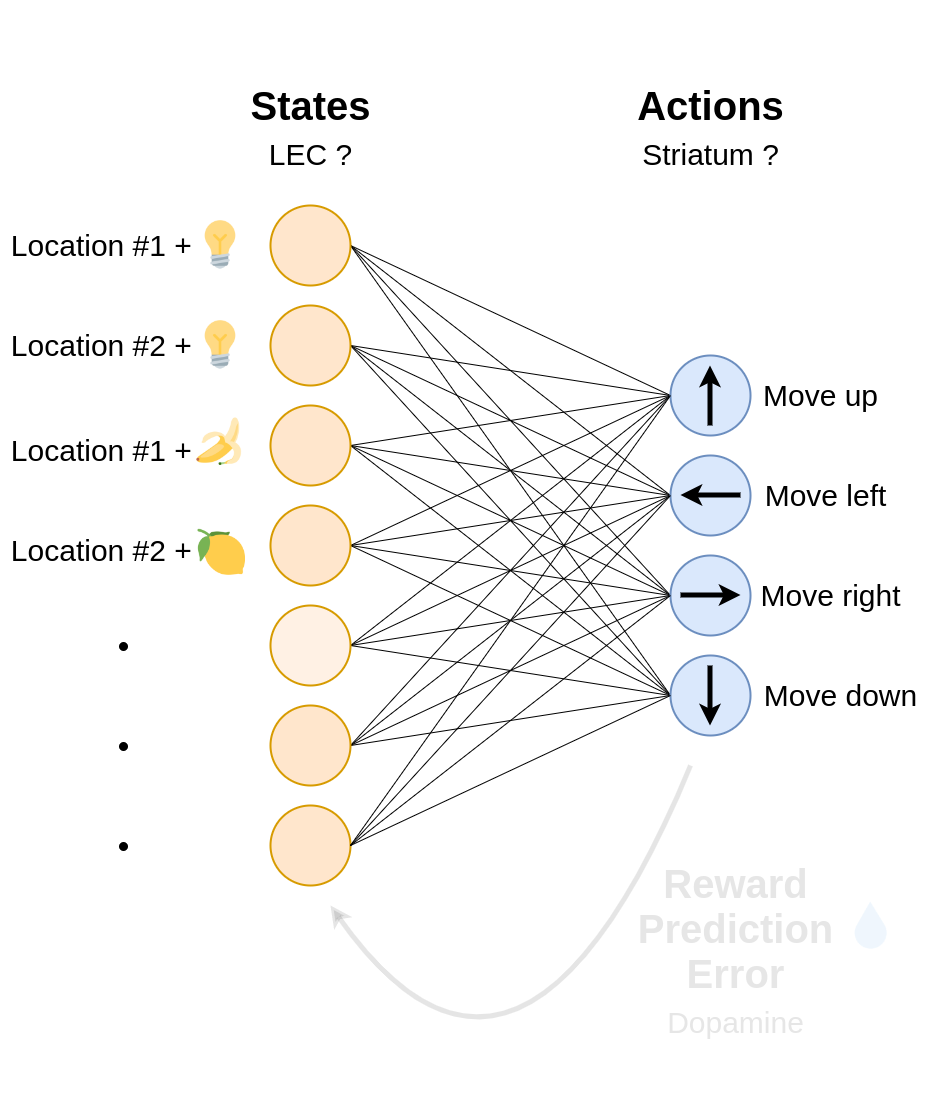
\includegraphics[height=\textheight]{img/RL_mapping-1.drawio.png}};
\end{tikzpicture}
\end{frame}
\begin{frame}[label={sec:org713c999}]{RL maps states to actions}
\center
\addtocounter{framenumber}{-1}
\begin{tikzpicture}
    \node[anchor=south west,inner sep=0] (image) at (0,0) {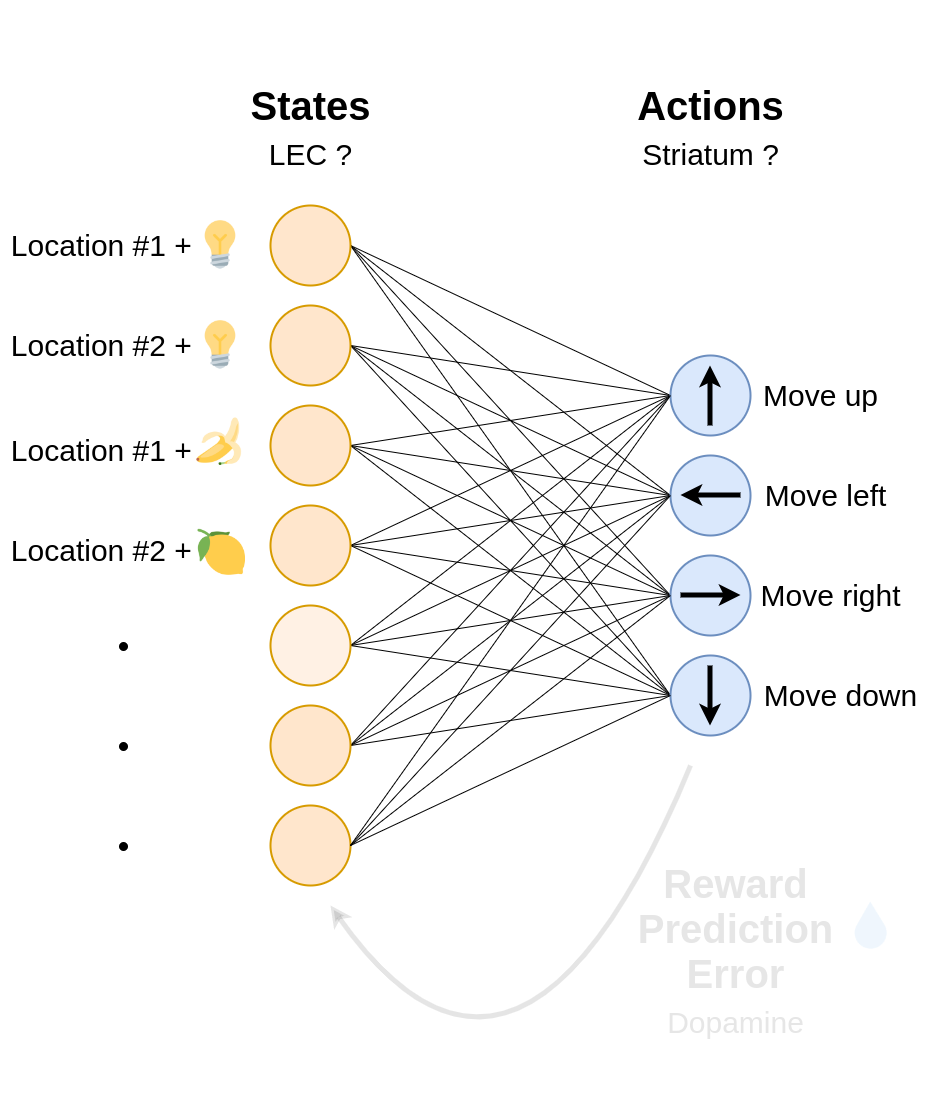
\includegraphics[height=\textheight]{img/RL_mapping-1.drawio.png}};
    \draw[RedBrown,ultra thick,rounded corners] (0,4) rectangle (3,4.7);
\end{tikzpicture}
\end{frame}
\begin{frame}[label={sec:org899ec21}]{RL maps states to actions}
\addtocounter{framenumber}{-1}
\center
\begin{tikzpicture}
    \node[anchor=south west,inner sep=0] (image) at (0,0) {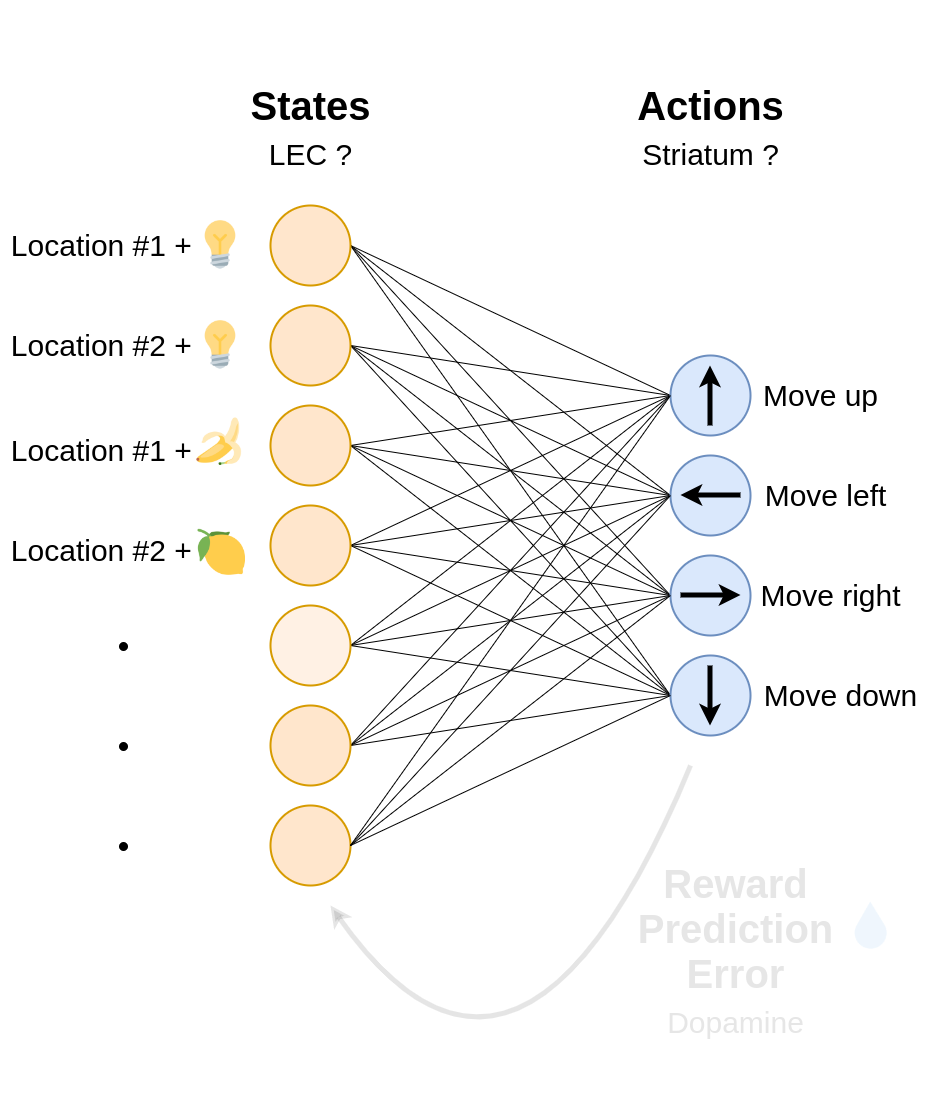
\includegraphics[height=\textheight]{img/RL_mapping-1.drawio.png}};
    \draw[RedBrown,ultra thick,rounded corners] (4.5,3.5) rectangle (7,4.5);
\end{tikzpicture}
\end{frame}
\begin{frame}[label={sec:org3cfb63f}]{RL maps states to actions}
\addtocounter{framenumber}{-1}
\center
\begin{tikzpicture}
    \node[anchor=south west,inner sep=0] (image) at (0,0) {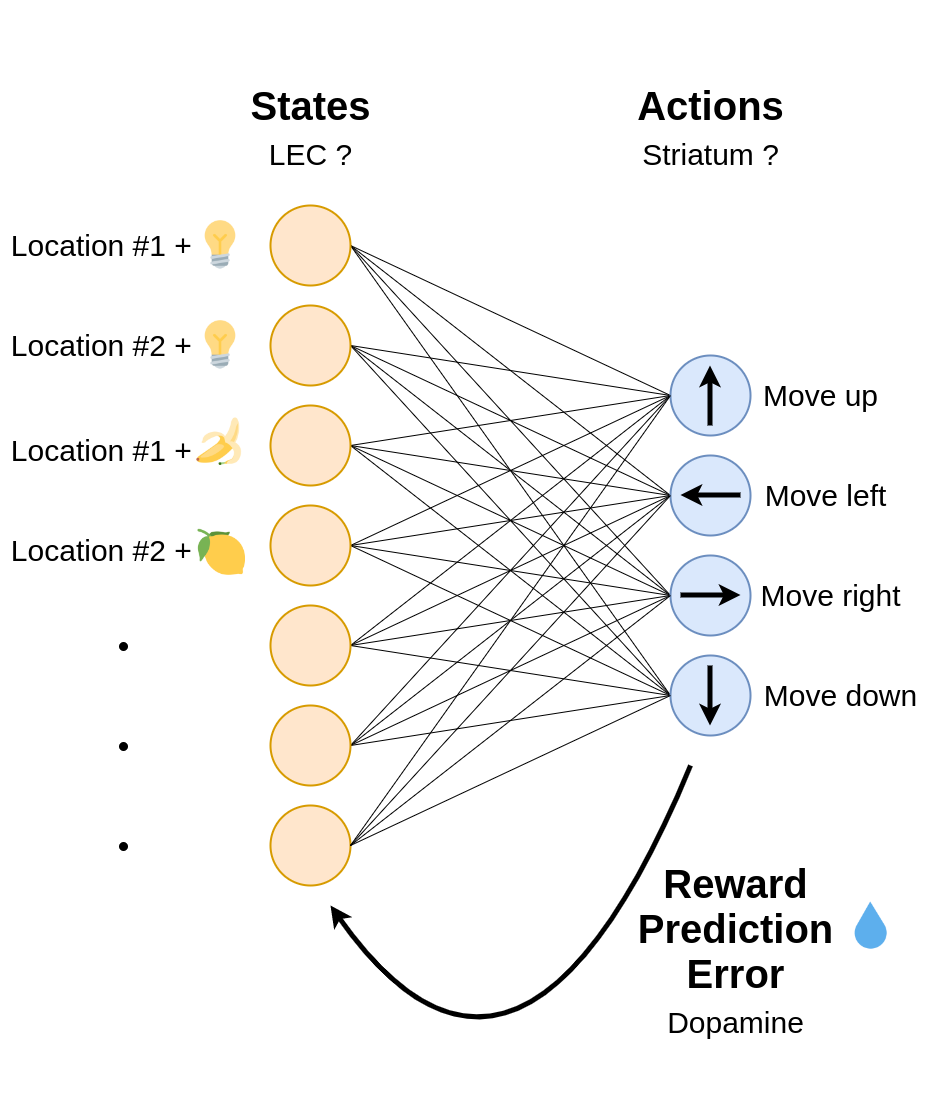
\includegraphics[height=\textheight]{img/RL_mapping-all.drawio.png}};
    \draw[RedBrown,ultra thick,rounded corners] (4.5,0.5) rectangle (7,2.5);
\end{tikzpicture}
\end{frame}
\begin{frame}[label={sec:orgc2f5272}]{RL maps states to actions}
\addtocounter{framenumber}{-1}
\center
\begin{tikzpicture}
    \node[anchor=south west,inner sep=0] (image) at (0,0) {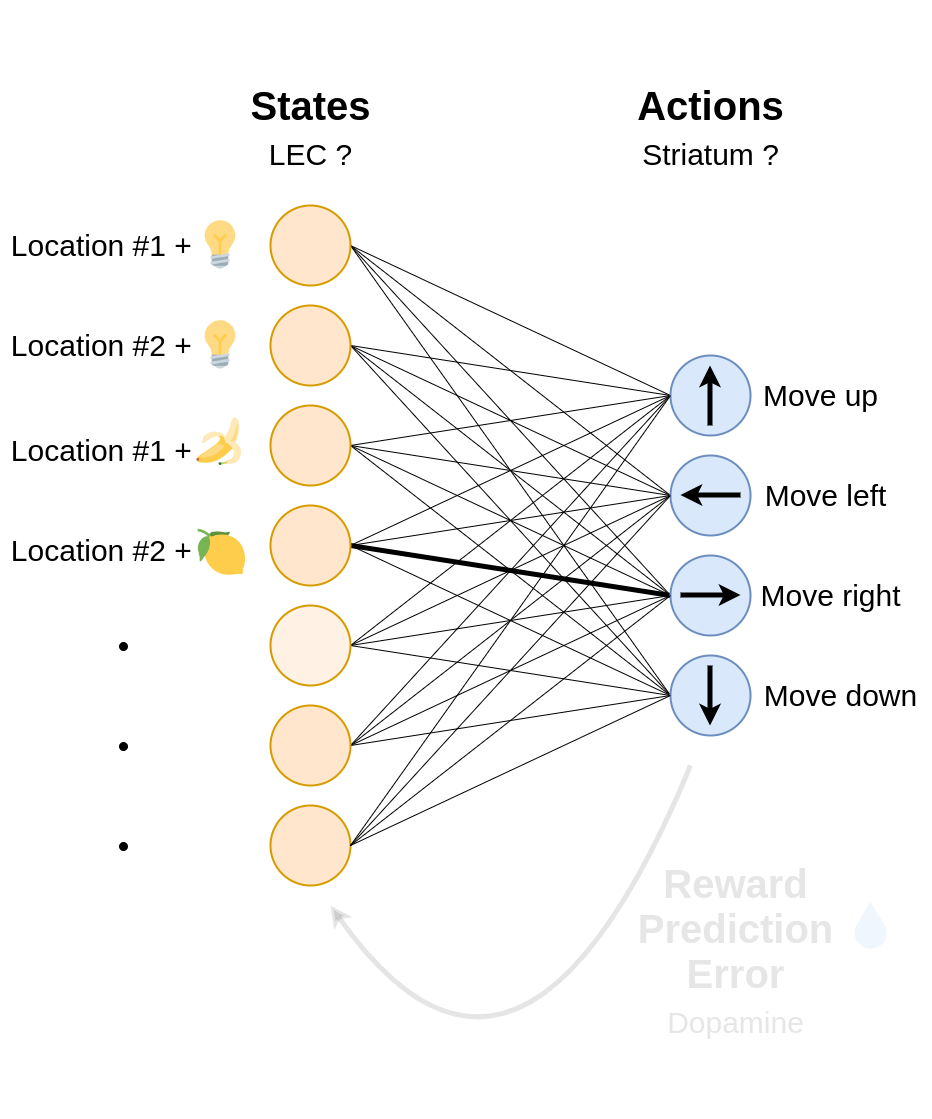
\includegraphics[height=\textheight]{img/RL_mapping-2.drawio.png}};
    \draw[RedBrown,ultra thick,rounded corners] (0,4) rectangle (3,4.7);
    \draw[RedBrown,ultra thick,rounded corners] (4.5,3.5) rectangle (7,4.5);
\end{tikzpicture}
\end{frame}
\begin{frame}[label={sec:orgb5e9474},standout]{~}
\raggedright
Which representations are needed by the brain to learn a place-odor association task ?
\end{frame}
\begin{frame}[label={sec:org88edbee}]{The joint representation encodes odor + location}
\begin{columns}
\begin{column}{0.33\columnwidth}
\begin{center}
Location only
\end{center}
\begin{center}
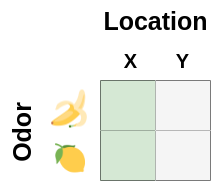
\includegraphics[width=.9\linewidth]{img/joint-repr-location.drawio.png}
\end{center}
\end{column}
\begin{column}{0.33\columnwidth}
\end{column}
\begin{column}{0.33\columnwidth}
\end{column}
\end{columns}
\end{frame}
\begin{frame}[label={sec:orge52cfca}]{The joint representation encodes odor + location}
\addtocounter{framenumber}{-1}
\begin{columns}
\begin{column}{0.33\columnwidth}
\begin{center}
Location only
\end{center}
\begin{center}
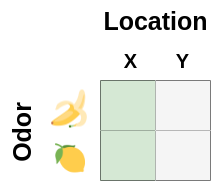
\includegraphics[width=.9\linewidth]{img/joint-repr-location.drawio.png}
\end{center}
\end{column}
\begin{column}{0.33\columnwidth}
\begin{center}
Odor only
\end{center}
\begin{center}
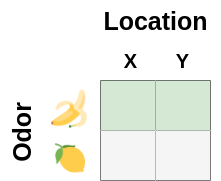
\includegraphics[width=.9\linewidth]{img/joint-repr-odor.drawio.png}
\end{center}
\end{column}
\begin{column}{0.33\columnwidth}
\end{column}
\end{columns}
\end{frame}
\begin{frame}[label={sec:org01c8ef6}]{The joint representation encodes odor + location}
\addtocounter{framenumber}{-1}
\begin{columns}
\begin{column}{0.33\columnwidth}
\begin{center}
Location only
\end{center}
\begin{center}
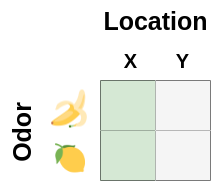
\includegraphics[width=.9\linewidth]{img/joint-repr-location.drawio.png}
\end{center}
\end{column}
\begin{column}{0.33\columnwidth}
\begin{center}
Odor only
\end{center}
\begin{center}
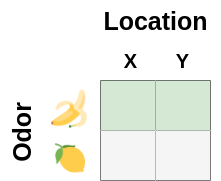
\includegraphics[width=.9\linewidth]{img/joint-repr-odor.drawio.png}
\end{center}
\end{column}
\begin{column}{0.33\columnwidth}
\begin{center}
Joint
\end{center}
\begin{center}
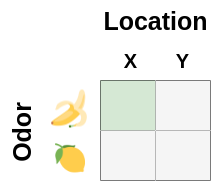
\includegraphics[width=.9\linewidth]{img/joint-repr-joint.drawio.png}
\end{center}
\end{column}
\end{columns}
\end{frame}
\section{Modeling \& preliminary results}
\label{sec:org0dcc403}
\begin{frame}[label={sec:org072e433}]{The model}
\begin{columns}
\begin{column}{0.5\columnwidth}
\center
Allocentric
\begin{center}
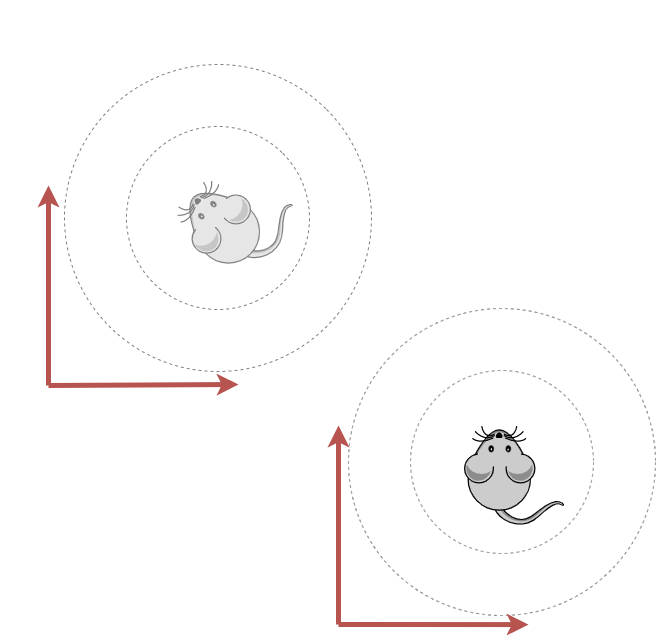
\includegraphics[height=0.2\textheight]{img/ego-vs-allo-allo.drawio.png}
\end{center}
\begin{center}
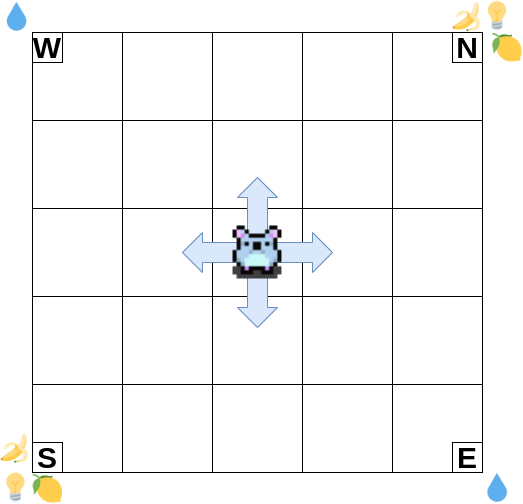
\includegraphics[width=0.9\textwidth]{img/RL_env-allo-model.drawio.png}
\end{center}
\end{column}
\begin{column}{0.5\columnwidth}
\end{column}
\end{columns}
\end{frame}
\begin{frame}[label={sec:org6f58a3c}]{The model}
\addtocounter{framenumber}{-1}
\begin{columns}
\begin{column}{0.5\columnwidth}
\center
Allocentric
\begin{center}
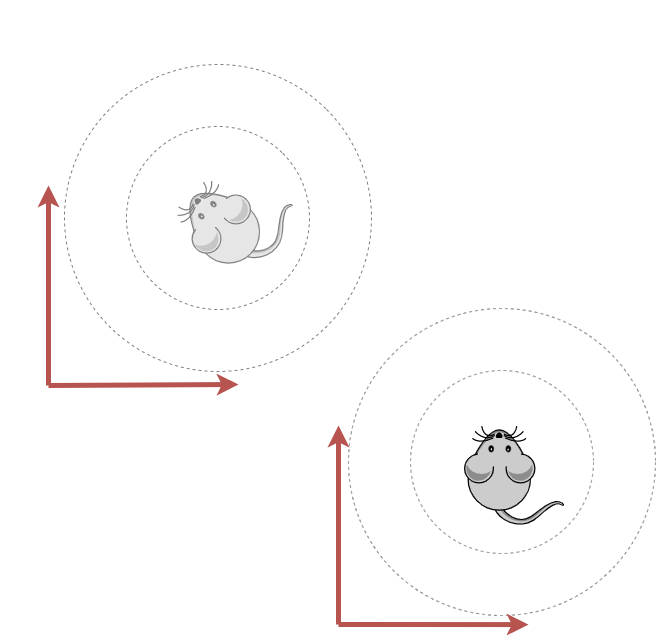
\includegraphics[height=0.2\textheight]{img/ego-vs-allo-allo.drawio.png}
\end{center}
\begin{center}
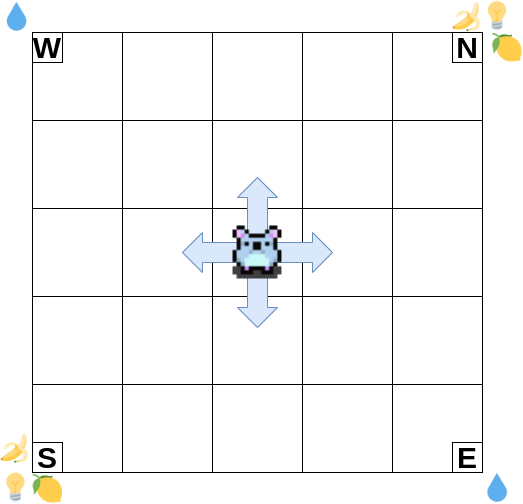
\includegraphics[width=0.9\textwidth]{img/RL_env-allo-model.drawio.png}
\end{center}
\end{column}
\begin{column}{0.5\columnwidth}
\center
Egocentric
\begin{center}
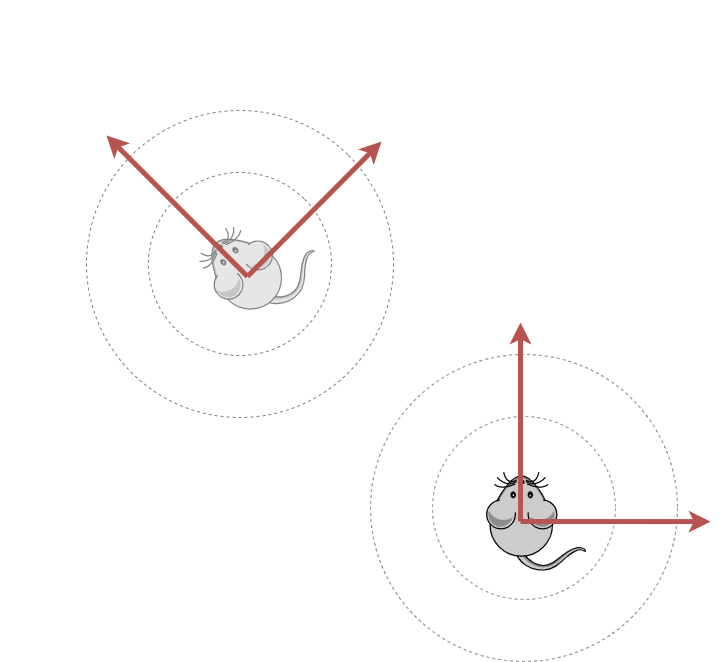
\includegraphics[height=0.2\textheight]{img/ego-vs-allo-ego.drawio.png}
\end{center}
\begin{center}
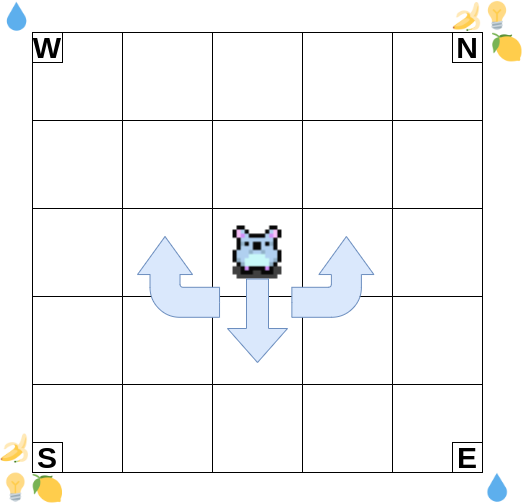
\includegraphics[width=0.9\textwidth]{img/RL_env-ego-model.drawio.png}
\end{center}
\end{column}
\end{columns}
\end{frame}
\begin{frame}[label={sec:org7e98144}]{Maximizing rewards}
\begin{columns}
\begin{column}[t]{0.5\columnwidth}
\begin{center}
Without joint representation
\end{center}
\begin{center}
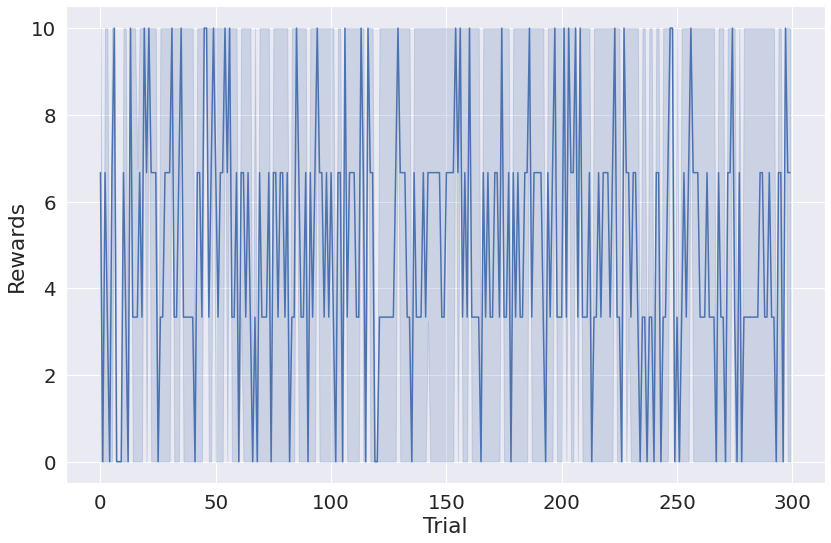
\includegraphics[width=\textwidth]{img/rewards-allo-no-joint-repr.png}
\end{center}
\(\to\) The agent doesn't learn
\end{column}
\begin{column}[t]{0.5\columnwidth}
\begin{center}
With joint representation
\end{center}
\begin{center}
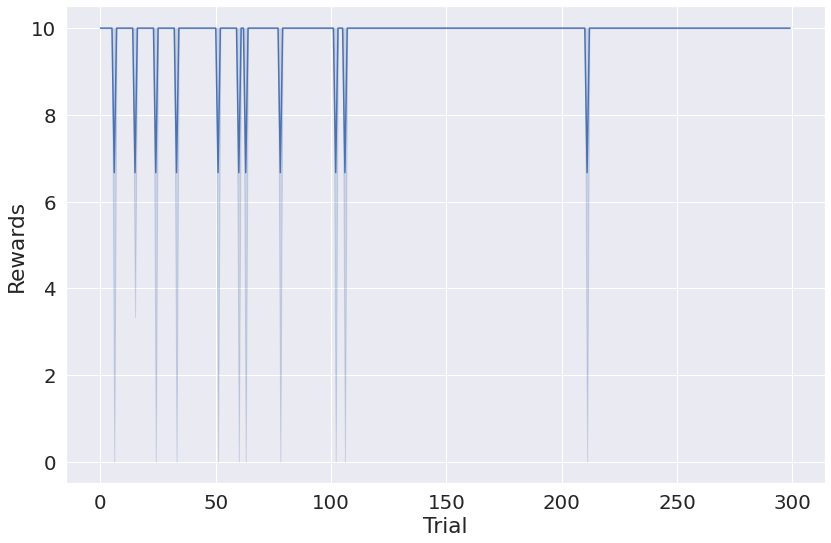
\includegraphics[width=\textwidth]{img/rewards-allo-joint-repr.png}
\end{center}
\(\to\) The agent learns to solve the task
\end{column}
\end{columns}
\end{frame}

\begin{frame}[label={sec:orgf68fe6e}]{Minimizing the number of steps to solve the task}
\begin{columns}
\begin{column}[t]{0.5\columnwidth}
\begin{center}
Without joint representation
\end{center}
\begin{center}
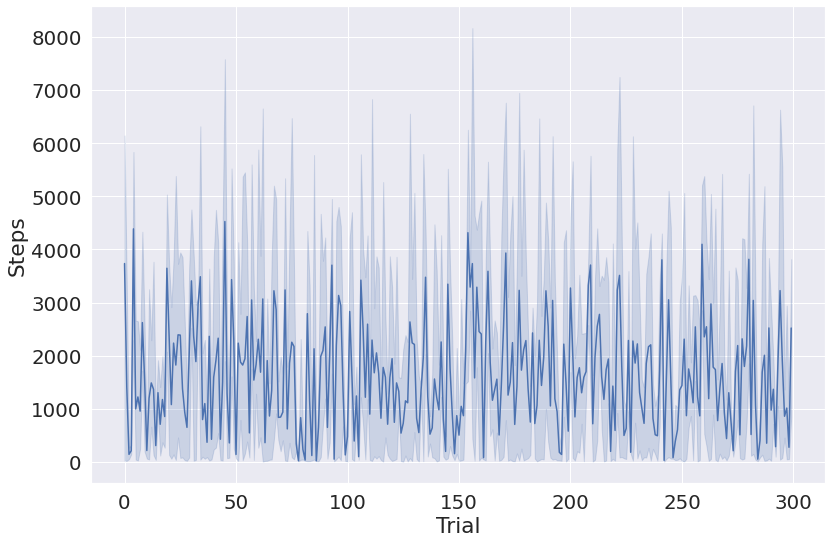
\includegraphics[width=\textwidth]{img/steps-allo-no-joint-repr.png}
\end{center}
\(\to\) The agent doesn't learn
\end{column}
\begin{column}[t]{0.5\columnwidth}
\begin{center}
With joint representation
\end{center}
\begin{center}
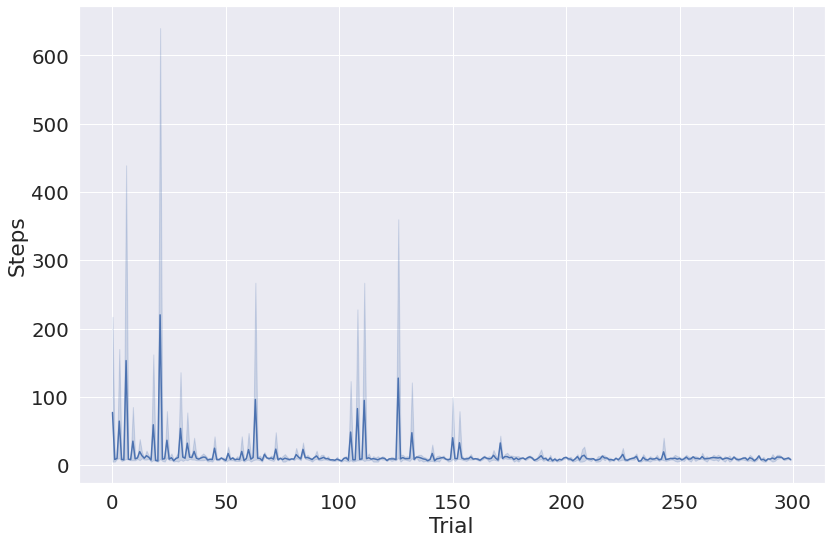
\includegraphics[width=\textwidth]{img/steps-allo-joint-repr.png}
\end{center}
\(\to\) The agent learns to solve the task
\end{column}
\end{columns}
\end{frame}

\begin{frame}[label={sec:orga9301f0}]{What policy did the agent learned ?}
\vspace{-7em}
\begin{columns}
\begin{column}[t]{0.5\columnwidth}
\begin{center}
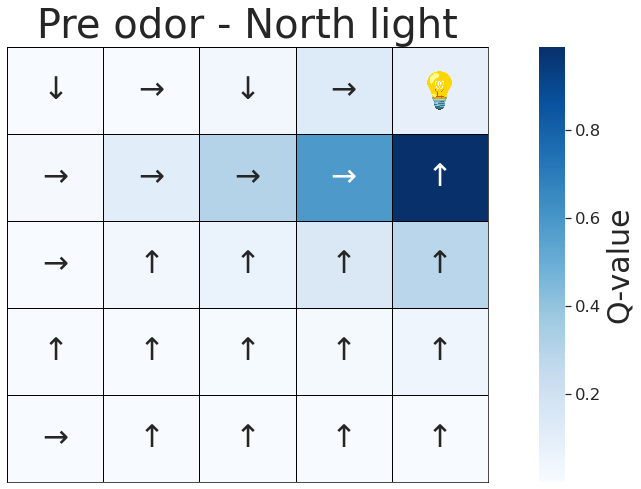
\includegraphics[height=0.4\textheight]{img/policy-allo-north-light.png}
\end{center}
\end{column}
\begin{column}[t]{0.5\columnwidth}
\begin{center}
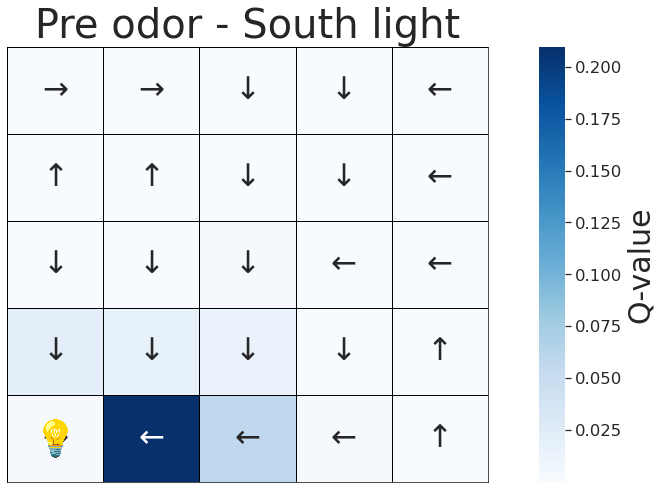
\includegraphics[height=0.4\textheight]{img/policy-allo-south-light.png}
\end{center}
\end{column}
\end{columns}
\end{frame}
\begin{frame}[label={sec:orgf1093f7}]{What policy did the agent learned ?}
\addtocounter{framenumber}{-1}
\begin{columns}
\begin{column}[t]{0.5\columnwidth}
\begin{center}
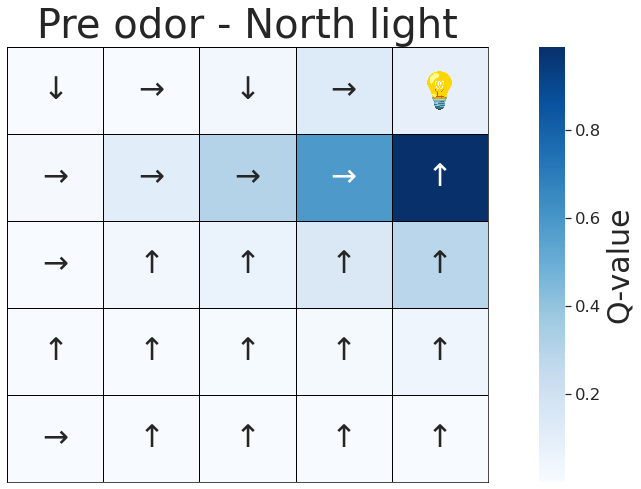
\includegraphics[height=0.4\textheight]{img/policy-allo-north-light.png}
\end{center}
\begin{center}
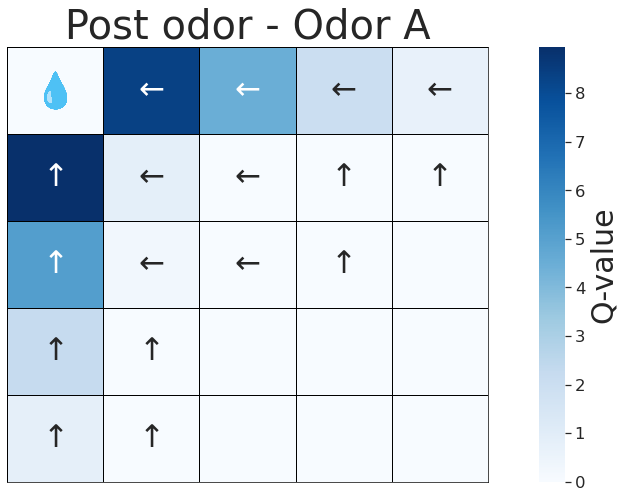
\includegraphics[height=0.4\textheight]{img/policy-allo-odor-A.png}
\end{center}
\end{column}
\begin{column}[t]{0.5\columnwidth}
\begin{center}
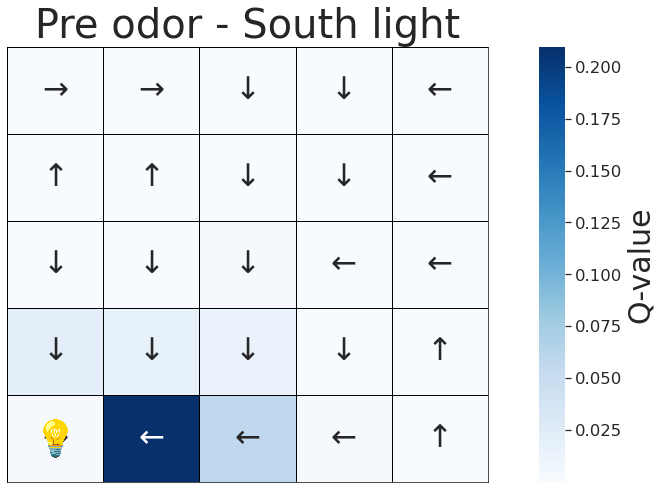
\includegraphics[height=0.4\textheight]{img/policy-allo-south-light.png}
\end{center}
\begin{center}
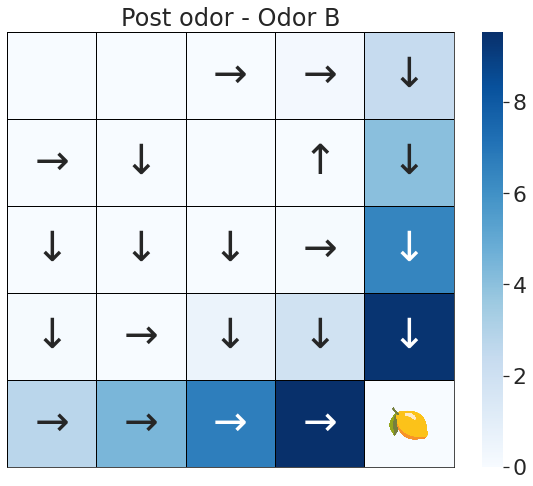
\includegraphics[height=0.4\textheight]{img/policy-allo-odor-B.png}
\end{center}
\begin{textblock}{0.2}(0.29,0.525)%

\includegraphics[height=1em]{img/banana.png}
\end{textblock}
\begin{textblock}{0.2}(0.855,0.525)%

\includegraphics[height=1em]{img/lemon.png}
\end{textblock}
\end{column}
\end{columns}
\end{frame}
\section{Next steps}
\label{sec:org2483366}
\begin{frame}[label={sec:org67d5dbf}]{Our RL model so far}
\begin{columns}
\begin{column}[t]{0.55\columnwidth}
% \usepackage{fontawesome5}
\usetikzlibrary{positioning,fit,arrows}


\tikzset{
    %Define standard arrow tip
    >=latex,
    %Define style for boxes
    punkt/.style={
           rectangle,
           rounded corners,
           draw=black, very thick,
           text width=7.5em,
           minimum height=2em,
           text centered},
    % Define arrow style
    pil/.style={
           ->,
           thick,}
}

\begin{adjustbox}{max width=\textwidth, keepaspectratio}
    \begin{tikzpicture}[node distance=3em, auto,]
     %nodes
        \node (center) {};
        \node[punkt, above=of center] (agent) {Agent \faIcon{robot}};
        % \node at (0,3.7) {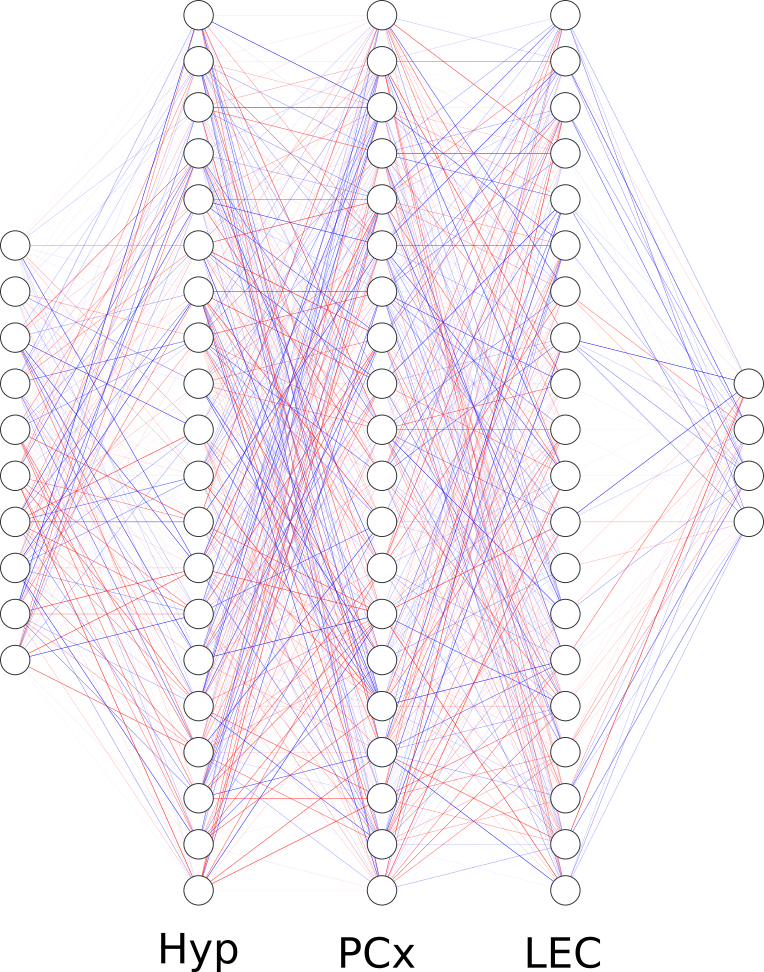
\includegraphics[height=6em]{./img/nn.svg.png}};
        \node [above=-0.2em of agent] {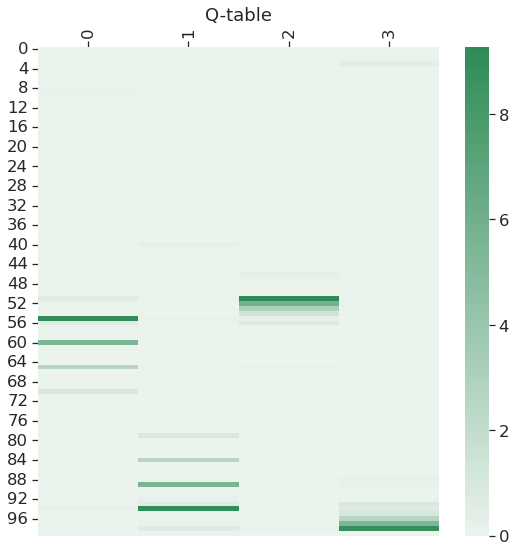
\includegraphics[height=8em]{./img/Q-table.png}};
        \node[punkt,below=of center] (environment) {Environment \faIcon{globe}};
        \node[right=8em of center, align=center] (action) {Action\\$a_t$};
        \node[left=8em of center, align=center] (state_reward) {State, Reward\\$s_t$, $r_t$};
        \node [below=-0.2em of environment] {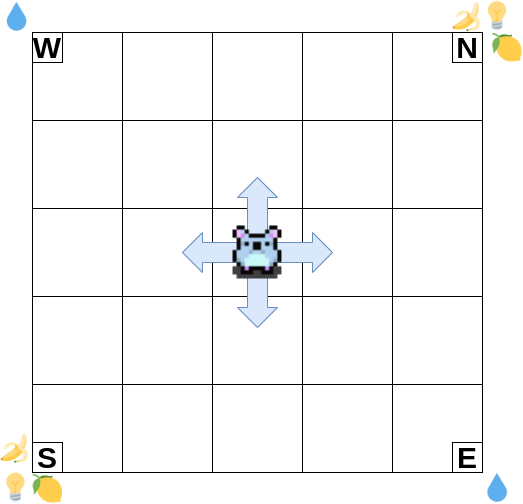
\includegraphics[height=8em]{./img/RL_env-allo-model.drawio.png}};

        \path[pil]
        (state_reward.east) edge [->, bend left=45] node {} (agent.west)
        (environment.west) edge [- , bend left=45] node {} (state_reward.east)
        (action.west) edge [->, bend left=45] node {} (environment.east)
        (agent.east) edge [-, bend left=45] node {} (action.west);
    \end{tikzpicture}
\end{adjustbox}
\end{column}

\begin{column}[t]{0.45\columnwidth}
\footnotesize
\begin{itemize}
\item Tabular model that maps states to actions
\item No generalization \(\to\)~each state needs to be visited by the agent to compute a prediction of getting a future reward
\end{itemize}
\end{column}
\end{columns}
\end{frame}

\begin{frame}[label={sec:org4b5aa01}]{Next step : from tabular RL to deep RL}
\begin{columns}
\begin{column}[t]{0.55\columnwidth}
% \usepackage{fontawesome5}
\usetikzlibrary{positioning,fit,arrows}


\tikzset{
    %Define standard arrow tip
    >=latex,
    %Define style for boxes
    punkt/.style={
           rectangle,
           rounded corners,
           draw=black, very thick,
           text width=7.5em,
           minimum height=2em,
           text centered},
    % Define arrow style
    pil/.style={
           ->,
           thick,}
}

\begin{adjustbox}{max width=\textwidth, keepaspectratio}
    \begin{tikzpicture}[node distance=3em, auto,]
     %nodes
        \node (center) {};
        \node[punkt, above=of center] (agent) {Agent \faIcon{robot}};
        % \node at (0,3.7) {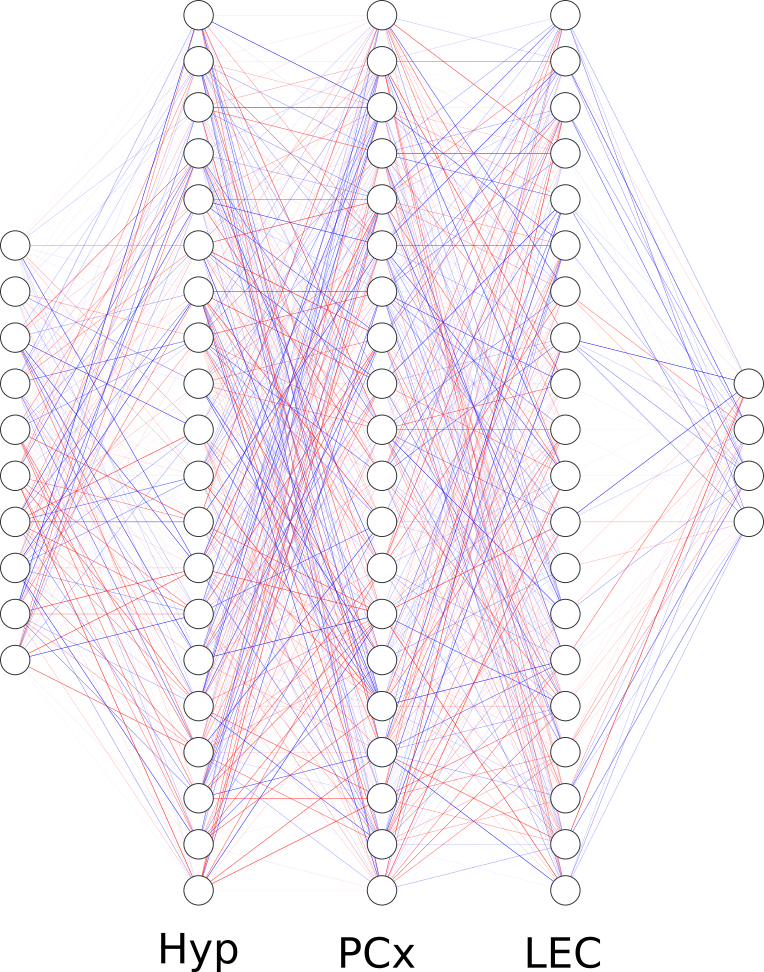
\includegraphics[height=6em]{./img/nn.svg.png}};
        \node [above=-0.2em of agent] {\includegraphics[height=8em]{./img/nn.svg.png}};
        \node[punkt,below=of center] (environment) {Environment \faIcon{globe}};
        \node[right=8em of center, align=center] (action) {Action\\$a_t$};
        \node[left=8em of center, align=center] (state_reward) {State, Reward\\$s_t$, $r_t$};
        \node [below=-0.2em of environment] {\includegraphics[height=8em]{./img/RL_env-allo-model.drawio.png}};

        \path[pil]
        (state_reward.east) edge [->, bend left=45] node {} (agent.west)
        (environment.west) edge [- , bend left=45] node {} (state_reward.east)
        (action.west) edge [->, bend left=45] node {} (environment.east)
        (agent.east) edge [-, bend left=45] node {} (action.west);
    \end{tikzpicture}
\end{adjustbox}
\end{column}

\begin{column}[t]{0.45\columnwidth}
\footnotesize
\begin{itemize}
\item Neural network does the mapping from states to actions
\item Learn to extract features/representations from the simulation data
\item Better generalization \(\to\)~the agent does not need to visit each state to compute a prediction of getting a future reward
\end{itemize}
\end{column}
\end{columns}
\end{frame}
\begin{frame}[label={sec:orgb6c045b}]{What types of representations are in use to solve an odor-place association task ?}
\begin{center}
\includegraphics[height=0.4\textheight]{img/exp-vs-simu.drawio.png}
\end{center}
\vspace{-3em}
\begin{columns}
\begin{column}[t]{0.5\columnwidth}
\begin{center}
\textbf{Experimental data}
\end{center}
\(\to\) Look for candidate patterns in the data: place cells, grid cells,\dots{}?
\end{column}
\begin{column}[t]{0.5\columnwidth}
\begin{center}
\textbf{Simulation}
\end{center}
\(\to\) Compare the experimental data with the representations learned from scratch by the neural network

% \begin{textblock}{5}(-8.5,0.5)
% \begin{minipage}[t]{3em}
% \center
% \includegraphics[height=2em]{img/matt-nassar.jpg}\\
% \scriptsize
% Matt Nassar
% \end{minipage}
% \begin{minipage}[t]{3em}
% \center
% \includegraphics[height=2em]{img/niloufar-razmi.jpeg}\\
% \scriptsize
% Niloufar Razmi
% \end{minipage}
% \end{textblock}
\end{column}
\end{columns}
\end{frame}

\begin{frame}[<+->][label={sec:org03ce384}]{Summary}
\begin{itemize}
\item LEC as candidate brain area for studying how \alert{odor} \& \alert{place} information are integrated in the brain
\item We use Reinforcement Learning to model behavior involving rewards and learning
\item The \alert{joint representation} is needed to solve an odor-place association task
\item We expect to use Deep Reinforcement Learning to investigate other types of representations that may be at play
\end{itemize}
\end{frame}
\section*{Acknowledgments}
\label{sec:orgdbc1dec}
{%
\setbeamertemplate{background canvas}{\includegraphics[height=\paperheight]{img/grand-canyon.JPG}}
\begin{frame}[fragile,t, plain]{Acknowledgments}
    \addtocounter{framenumber}{-1}
    %\vspace{1em}
    \begin{columns}[T]
        \begin{column}{0.5\textwidth}
            \begin{tcolorbox}[opacityfill=0.1, arc=0mm, size=fbox, coltext=white, colback=black, colframe=black]
                \small
                \centering
                \textbf{Fleischmann lab}
                \begin{itemize}[noitemsep, before=\color{white}\bfseries]
                    \scriptsize
                    %{\transparent{0.5}\colorbox{white}{%
                    \item Alexander Fleischmann
                    \item Keeley Baker
                    \item Olivia Mckissick
                    \item Tuan Pham
                    \item Simon Daste
                    \item Max Seppo
                    %\item \colorbox{white}{\transparent{0.2}Sara Zeppilli}
                    \item Sara Zeppilli
                    \item Nell Klimpert
                    \item Erin Meyers
                    \item Eseosa Uwaifo
                    \item Camille Donoho
                    \item Timothy Pyon
                \end{itemize}
            \end{tcolorbox}
            %\vspace{5em}
            \includegraphics[height=1.5cm]{img/qr-code.png}\\
            %\colorbox{white}{\footnotesize\transparent{0.5}https://reduced.to/tn9x6}
        \end{column}

        \begin{column}{0.5\textwidth}
            \begin{tcolorbox}[opacityfill=0.1, arc=0mm, size=fbox, coltext=white, colback=black, colframe=black]
                \small
                \centering
                \textbf{Collaborations}
                \begin{itemize}[noitemsep, before=\color{white}\bfseries]
                    \scriptsize
                    \item Matt Nassar
                    \item Jason Ritt
                    \item Niloufar Razmi
                \end{itemize}
            \end{tcolorbox}
        \end{column}
    \end{columns}
\end{frame}
}
\section{Backup}
\label{sec:org8a5de74}
\begin{frame}[label={sec:orga6fdf96}]{Policy learned in the egocentric version}
\addtocounter{framenumber}{-1}
\begin{center}
\includegraphics[width=.9\linewidth]{img/policy-ego-joint-repr.png}
\end{center}
\end{frame}
\end{document}
